\section{\bpfcontain{} Design and Implementation}
\label{sec:design}

\todo{Introduce \bpfcontain{} and talk about how it attempts to solve container security}

\subsection{Design Goals}

Five specific goals informed the design of \bpfcontain{}'s policy language and
enforcement mechanism, enumerated below as Design Goals \ref{d:1} to \ref{d:5}.
%Note that there is a natural interplay between some of these design goals, while
%others are typically perceived as being in contention (specifically usability
%and security). In cases of conflict, it is essential to strike a careful balance
%between each property.

\begin{enumerate}[label=\bfseries D\arabic*., ref=D\arabic*, labelindent=1em]
  \item \label{d:1} \textsc{Usability.}
    \bpfcontain{}'s basic functionality should not impose unnecessary usability
    barriers on end-users.  Its policy language should be easy to understand and
    semantically meaningful to users without significant security knowledge. To
    accomplish this goal, \bpfcontain{} takes some inspiration from other high-level
    policy languages for containerized applications, such as those used in
    Snapcraft \cite{snap}.

  \item \label{d:2} \textsc{Configurability.}
    It should be easy for an end-user to reconfigure policy to match their
    specific use case, without worrying about the underlying details of the
    operating system or the policy enforcement mechanism. It should be possible
    to use \bpfcontain{} to restrict specific unwanted behaviour in a given
    application without needing to write a rigorous security policy from
    scratch.

  \item \label{d:3} \textsc{Transparency.}
    Containing an application using \bpfcontain{} should not require modifying the
    application's source code or running the application using a privileged SUID
    (Set User ID root) binary. \bpfcontain{} should be entirely agnostic to the rest
    of the system and should not interfere with its regular use.

  \item \label{d:4} \textsc{Adoptability.}
    \bpfcontain{} should be adoptable across a wide variety of system configurations
    and should not negatively impact the running system. It should be possible
    to deploy \bpfcontain{} in a production environment without impacting system
    stability and robustness or exposing the system to new security
    vulnerabilities. \bpfcontain{} relies on the underlying properties of its eBPF
    implementation to achieve its adoptability guarantees.

  \item \label{d:5} \textsc{Security.}
    \bpfcontain{} should be built from the ground up with security in mind. In
    particular, security should not be an opt-in feature and \bpfcontain{} should
    adhere to the principle of least privilege \cite{saltzer1975_protection} by
    default. It should be easy to tune a \bpfcontain{} policy to respond to new
    threats.
\end{enumerate}

\subsection{Architectural Overview}
\label{sub:architecture}

\bpfcontain{} consists of both userspace and kernelspace components, which interact co-operatively to implement its policy enforcement mechanism. Roughly, its architecture (depicted in \Cref{fig:architecture}) can be broken down into the following four components:
\begin{enumerate}[label=\bfseries C\arabic*., ref=C\arabic*, labelindent=1em]
  \item \label{c:1}
    A privileged daemon, responsible for loading and managing the lifecycle of eBPF programs and maps and logging security events to userspace.

  \item \label{c:2}
    A small shared library and unprivileged wrapper application used to initiate confinement.

  \item \label{c:3}
  A set of eBPF programs, running in kernelspace. These programs are attached to LSM hooks in the kernel as well as the shared library in \ref{c:2}.

  \item \label{c:4}
  A set of eBPF maps, special data structures which allow bidirectional communication between userspace and kernelspace. These maps are used to track the state of running containers and store the active security policy for each container.
\end{enumerate}

\begin{figure}[htb]
  \centering
  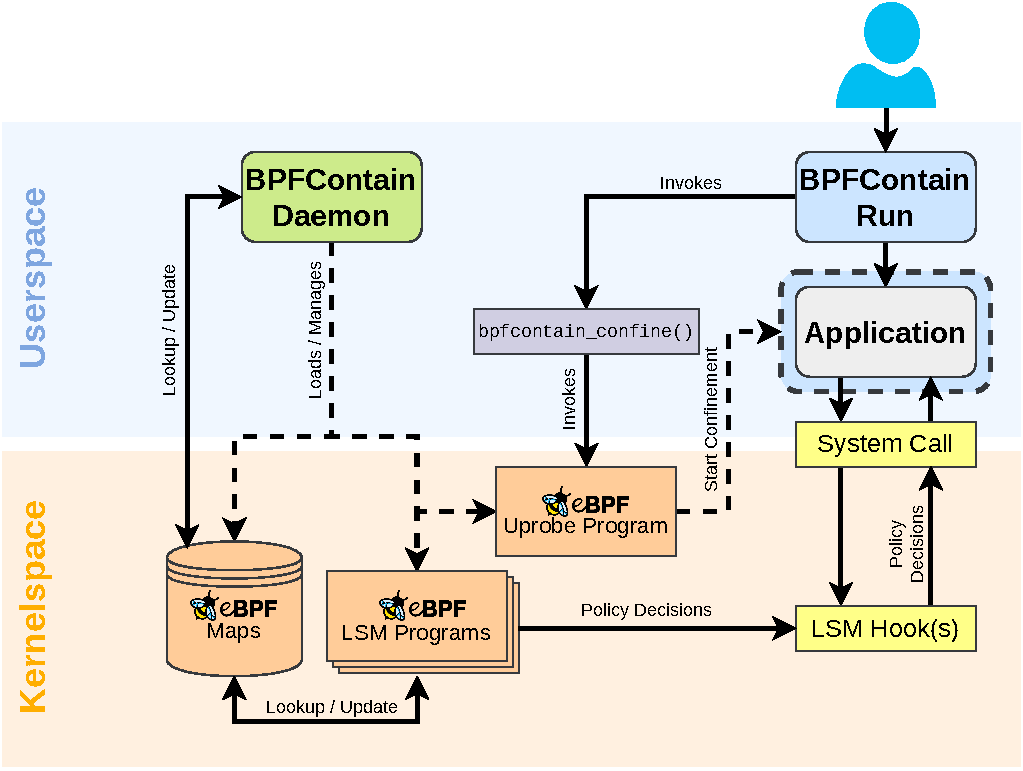
\includegraphics[width=0.8\linewidth]{figs/architecture.pdf}
  \caption{
    A diagram of \bpfcontain{}'s architecture. The privileged daemon (green) is responsible for loading the necessary eBPF maps and programs (orange) into the kernel and managing their lifecycle. The user starts a container by executing an unprivileged wrapper application (blue), which invokes the \texttt{bpfcontain\_confine} library call (purple), trapping to a special eBPF program that associates the process group with the right policy.  When the confined application (grey) makes a system call to request access to a sensitive resource, the kernel invokes one or more LSM hooks (yellow), which trap to corresponding eBPF LSM programs that make the correct policy decision.
  }%
  \label{fig:architecture}
\end{figure}

In userspace, \bpfcontain{} is implemented as a privileged daemon based on the bcc \cite{bcc} eBPF framework for Python. The daemon is responsible for loading \bpfcontain{}'s eBPF programs and maps and logging security events to userspace, such as policy violations.  When it first starts, the daemon invokes a series of \texttt{bpf(2)} system calls to load its eBPF programs and maps into the kernel. After loading all eBPF programs and maps, the daemon then parses, translates, and loads each per-container policy file into several eBPF maps.

For the bulk of its policy enforcement \bpfcontain{} leverages the KRSI (kernel runtime security instrumentation) patch merged by KP Singh~\cite{singh2019_krsi,corbet2019_krsi} into the Linux 5.7 kernel. This patch enables eBPF programs to be attached to LSM hooks at runtime, making policy decisions and log security events.  These programs work cooperatively with each other and with any other LSMs running on the system to come to a policy decision. When an event fires, the LSM programs query policy from policy maps to come to a decision. This dynamic runtime policy enforcement is at the core of \bpfcontain{}'s flexible container security approach.

\subsection{\bpfcontain{} Policy}
\label{sub:policy}

\bpfcontain{} policy consists of simple manifests written in YAML \cite{yaml}, a human-readable data serialization language based on key-value pairs.  Each \bpfcontain{} container is associated with a manifest, which itself consists of a few lines of metadata followed by a set of \textit{rights} and \textit{restrictions}.  A \textit{right} specifies access that should be granted to a container, while a \textit{restriction} is used revoke access. While rights and restrictions may be combined at various granularities, a restriction always overrides a right of the same or coarser granularity. For instance, a right to access the root filesystem would be overridden by a restriction on the user's home directory. In practice, this allows the construction of nuanced policies that specify coarse-grained access with finer-grained exceptions.  \Cref{tab:accesses} describes the various access labels that can be used in \bpfcontain{} policy.

{
\small
\begin{longtable}[c]{llp{25em}}
  \caption{
    Access labels for \bpfcontain{} policy along with their parameters and descriptions. Square brackets denote an optional parameter.
  }
  \label{tab:accesses}\\
  \toprule
  Resource              & Parameters          & Description \\
  \midrule
  \endfirsthead
  \texttt{filesystem} & Mountpoint, [Access] &
    Grants or revokes access at the granularity of a filesystem mountpoint. Access defaults to read, write, append, chdir, create, and setattr, unless otherwise specified. An optional \texttt{readonly} flag grants read and chdir access. An optional \texttt{appendonly} flag grants read, append, setattr, create, and chdir access. \\
  \texttt{file}       & Pathname, Access  &
    Grants or revokes access at the granularity of individual files. Access must be specified as a string of access flags (see \Cref{tab:fs_policy}). \\
  \midrule
  \texttt{net-bind} &  &
    Grants or revokes access to the \texttt{CAP\_NET\_BIND\_SERVICE} POSIX capability, allowing the container to bind to privileged ports. \\
  \texttt{net-raw} &  &
    Grants or revokes access to the \texttt{CAP\_NET\_RAW} POSIX capability, allowing the container to use raw sockets. \\
  \texttt{net-broadcast} &  &
    Grants or revokes access to the \texttt{CAP\_NET\_BROADCAST} POSIX capability, allowing the container to broadcast and listen to multicast network traffic. \\
  \texttt{dac-override} &  &
    Grants or revokes access to the \texttt{CAP\_DAC\_OVERRIDE} POSIX capability, allowing the container to override discretionary access controls. \\
  \midrule
  \texttt{network}    & [Family], [Access] &
    Grants or revokes access to network communications. A specific address family and access pattern may optionally be specified. \\
  \texttt{ipc}        & Container           &
    Grants or revokes access to communicate with processes in \textit{another} \bpfcontain{} container. This covers all supported System V IPC categories as well as Unix sockets and signals. Both containers must mutually declare IPC access. \\
  \midrule
  \texttt{tty}        & [Access]            &
    Grants or revokes access to terminal devices. \\
  \texttt{pts}        & [Access]            &
    Grants or revokes access to pseudo-terminal devices. \\
  \texttt{video}      & [Access]            &
    Grants or revokes access to video devices. \\
  \texttt{sound}      & [Access]            &
    Grants or revokes access to sound devices. \\
  \texttt{graphics}   & [Access]            &
    Grants or revokes access to graphics devices. \\
  \texttt{random}   & [Access]            &
    Grants or revokes access to random and urandom devices. \\
  \multicolumn{3}{c}{...} \\
  \bottomrule
\end{longtable}
}

\bpfcontain{} provides three policy granularities for file access: filesystem rules, file rules, and device rules. A filesystem rule grants access to an entire filesystem, specified by providing the pathname of its mountpoint. For instance, a policy would specify access to the root filesystem with \texttt{filesystem /} and procfs with \texttt{filesystem /proc}. File rules specify access at the granularity of individual files and directories. Finally, coarse-grained device rules such as tty, pts, video, and sound specify access at the granularity of common character and block devices. Each file access rule supports 13 specific access categories (outlined in \Cref{tab:fs_policy}) which may be combined as necessary. Filesystem rules also support two coarse-grained access flags, \texttt{readonly} and \texttt{appendonly}, which act as shortcuts for commonly-used access flags for filesystems.

{
\small
\begin{longtable}[c]{llp{25em}}
  \caption{
    Access categories for filesystem and file policy.
  }
  \label{tab:fs_policy}\\
  \toprule
  Access             & Flag       & Description \\
  \midrule
  \endfirsthead
  Read               & \texttt{r} & The container may read the file. This does not apply to directories. \\
  Write              & \texttt{w} & The container may write to the file. This does not apply to directories. \\
  Execute            & \texttt{x} & The container may execute the file (via execve). This does not apply to directories. \\
  Append             & \texttt{a} & The container may append to the file (without overwriting existing contents). This does not apply to directories.\\
  Create             & \texttt{c} & The container may create new files in the directory. \\
  Rename             & \texttt{n} & The container may rename the file or directory. \\
  Delete             & \texttt{d} & The container may delete the file or directory. \\
  Change Directory   & \texttt{t} & The container may change directory into this directory. \\
  Set Attribute      & \texttt{s} & The container may set attributes on this file or directory. \\
  Change Permissions & \texttt{p} & The container may change permissions on the file or directory. \\
  Change Owner       & \texttt{o} & The container may change the owner of the file or directory \\
  Link               & \texttt{l} & The container may create a hard link to the corresponding inode. \\
  Execute Mapped     & \texttt{m} & The container may map the file into memory for execution (other \texttt{mmap} operations are governed normally by read, write, and append access). This allows policy to distinguish shared libraries from executables. \\
  \bottomrule
\end{longtable}
}

\bpfcontain{} defines four capability rules which are used to specify exceptions to its default-deny policy on POSIX capabilities. The \texttt{netbind} rule grants the ability to bind to privileged ports, the \texttt{netraw} rule grants the ability to use raw sockets, and the \texttt{netbroadcast} rule grants the ability to broadcast and listen to multicast network traffic. The \texttt{dac-override} rule grants the ability to override discretionary access controls on files. All other POSIX capabilities are implicitly denied and may not be overridden. Note that these capability rules may not be used to grant overpermission to a container---the underlying process must already have the actual capability to use it.

Network policy in \bpfcontain{} enforces at the socket level, across various granularities. The most basic network policy consists of a single rule \texttt{network} which grants coarse-grained access to the entire networking stack. A specific address family and level of access may also be specified for finer-grained policy. Network policy is closely related to IPC policy, which grants or revokes permission to perform interprocess communication between containers. Support IPC mechanisms include System V IPC, signals, and Unix sockets (which must also be declared under network policy). For inter-container IPC to be valid, \textit{both} containers must mutually declare IPC access to each other. In other words, if container $A$ wishes to perform IPC with container $B$, container $A$ must list an \lstinline[language=yaml]{ipc: B} right and container $B$ must also list an \lstinline[language=yaml]{ipc: A} right.

\todo{Maybe cover some policy examples}

\subsection{Launching a \bpfcontain{} Container}
\label{sub:launching}

To allow processes to request that they be placed into a container, \bpfcontain{} attaches a specialized eBPF program type called a \texttt{uprobe} (userspace probe) to a userspace library call, \texttt{bpfcontain\_confine}.  This function is a stub, whose only purpose is to trap to the uprobe---if it fails to trap the corresponding eBPF program (for example if \bpfcontain{} has not yet loaded its eBPF programs into the kernel), the function returns \texttt{-EAGAIN} to indicate that the caller should repeat the request. Attaching a \texttt{uprobe} to a library call in this way is a common eBPF design pattern, which effectively allows eBPF programs to make almost arbitrary extensions to the kernel's API.

When \texttt{bpfcontain\_confine} traps to its corresponding uprobe, the uprobe queries the current PID and associates that PID with a corresponding container ID. This container parameterizes \bpfcontain{}'s policy maps, allowing it to query the given container's correct policy. Subsequent forks associate newly created processes with the parent's container ID, assuring that the entire process subtree belongs to the same container. Once a process has been associated with a specific container ID, this association persists until the process exits, preventing the \texttt{bpfcontain\_confine} call from being abused to transition to another container profile.

From the user's perspective, running a \bpfcontain{} container is as simple as invoking the \texttt{bpfcontain run -n <name>} command. This command is a thin wrapper around the \texttt{bpfcontain\_confine} library call discussed above. Its only purpose is to invoke this library call, check for a successful invocation (using its return value), and then execute the command defined in the corresponding container manifest. See \Cref{fig:launch} for an overview of this process.

\begin{figure}[htb]
  \centering
  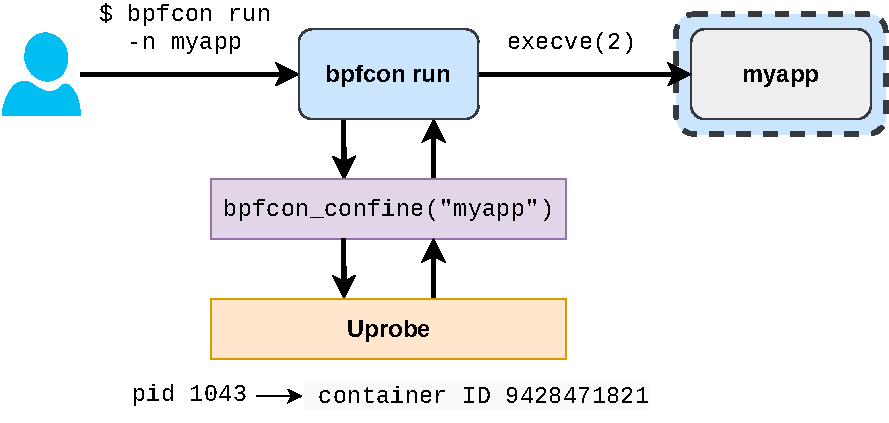
\includegraphics[width=0.6\linewidth]{figs/launch.pdf}
  \caption{Launching a \bpfcontain{} container.}%
  \label{fig:launch}
\end{figure}

\todo{Not sure if I really want to say this or not}
An important feature of \bpfcontain{} is that the \lstinline[language=c]|bpfcontain_confine| library call requires no additional operating system privileges to start confinement.  This notion of unprivileged confinement is a unique advantage over other container implementations in Linux.  Somewhat counter-intuitively, traditional container implementations often rely on binaries with escalated privileges (e.g.~setuid root) to set up proper confinement.  Failure to correctly drop these elevated privileges may result in \textit{escalation of privilege} in the host system, particularly if the confined process manages to escape the container.  By obviating this need for elevated privileges, \bpfcontain{} conforms with the principle of least privilege and improves its overall security.

As a side effect of \bpfcontain{}'s design, it is also possible for a generic application to invoke the \lstinline[language=c]|bpfcontain_confine| library call directly, eliminating the need to start the target application using the \texttt{bpfcontain run} wrapper. This notion of self-confinement enables application developers and package maintainers to ship \bpfcontain{} policy with their software and enforce it transparently to the end-user. Since \bpfcontain{} policy is designed to be readable and modifiable by end-users, a security policy shipped with an application could optionally be tuned by the user according to their specific needs.

\subsection{Policy Enforcement Mechanism}
\label{sub:enforcement}

%\bpfcontain{} only enforces security policy on processes which are currently
%associated with a container. The list of processes associated with a container
%is tracked using an eBPF map, which is updated whenever a process invokes the
%\texttt{bpfcontain\_confine} library call (assuming it is not already in
%a container), and whenever a process that is currently in a container forks
%itself. Once a process has been associated with a container, it remains
%associated with that container until it terminates.

Security policy in \bpfcontain{} falls into two categories: \textit{implicit} and \textit{explicit}. Explicit policy is per-container policy defined by the end-user in the container's manifest (see \Cref{sub:policy}). On the other hand, implicit policy comprises the set of sensible defaults which are applied and enforced for every container, regardless of its configuration. The vast majority of implicit \bpfcontain{} policy consists of behavioural restrictions, which prohibit a container from performing a set of dangerous actions which could be used to escape confinement, attack other containers, or negatively impact the host system. Conversely, other implicit policy grants a minimal set of rights to a container, including the ability to interact with its own procfs entries, communicate with other processes running in the same container, and access newly created files by processes within the container (e.g.~temporary files). \Cref{tab:implicit} describes each implicit policy category in \bpfcontain{}.

\begingroup
\small
\begin{longtable}[c]{llp{25em}}
  \caption{
    Implicit policy in \bpfcontain{}, which is enforced regardless of a container's manifest. Implicit restrictions generally correspond with resources which a well-behaved container should never need. Implicit rights permit certain sane behaviours, such as interprocess communication between processes \textit{within} a container. These rights effectively constitute exceptions to ordinary enforcement. Note that implicit rights may still be overridden by an explicit restriction specified in the container's manifest. A third category, implicit death, refers to accesses that cause \bpfcontain{} to send an uncatchable SIGKILL to the process.
  }
  \label{tab:implicit}\\
  \toprule
  Policy & Kind & Description \\
  \midrule
  \endfirsthead
  BPF & Restriction &
    A container is disallowed from making \textit{any} \texttt{bpf(2)} system calls. This restriction prevents a container from loading, unloading, and accessing any eBPF programs and maps, including those which belong to \bpfcontain{} itself. \\
  Ptrace & Restriction &
    A container may not use \texttt{ptrace(2)} to trace or control processes. \\
  Kernel Lockdown & Restriction &
    A container is subject to full Kernel Lockdown \cite{lockdown} restrictions, disabling all operations that could be used for arbitrary code execution in the kernel. \\
  Kernel Modules & Restriction &
    A container may not load any modules into the kernel. \\
  Kexec & Restriction &
    A container may not use \texttt{kexec}-family system calls to load new kernels. \\
  Shutdown & Restriction &
    A container may not shut down or reboot the system. \\
  Key Management & Restriction &
    A container may not interface with the kernel's key management mechanisms. \\
  Quotactl & Restriction &
    A container cannot use the \texttt{quotactl(2)} system call to bypass restrictions on resource consumption. \\
  Rlimit & Restriction &
    A container cannot use the \texttt{getrlimit(2)}, \texttt{setrlimit(2)}, or \texttt{prlimit(2)} system calls to get or set resource limits. \\
  Scheduler & Restriction &
    A container cannot inspect or modify process scheduling or I/O scheduling priority. \\
  Mount & Restriction &
    A container cannot mount, remount, unmount filesystems or move filesystem mounts. \\
  Pivot Root & Restriction &
    A container cannot pivot the root directory of a filesystem. \\
  Syslog & Restriction &
    A container cannot use the \texttt{syslog(2)} system call to access the kernel logs. \\
  Set Time & Restriction &
    A container cannot use the \texttt{settime(2)} system call to change the system time. \\
  \midrule
  Privilege Escalation & Death &
    To prevent kernel privilege escalation exploits which typically rely on forcing the execution of \texttt{commit\_creds} \cite{xin2018_container_security}, \bpfcontain{} will outright kill a contained process that invokes this function (outside of the execve code path) to try to escalate its privileges. \\
  \midrule
  IPC & Right &
    A process can always perform interprocess communication with another process within the same container. \\
  Procfs & Right &
    A process is granted full access to its own procfs entries, as well as those belonging to other processes within the same container. \\
  New Files & Right &
    A container is granted full access to any new files or directories that it creates. \\
  \bottomrule
\end{longtable}
\endgroup

Following the principle of least privilege \cite{saltzer1975_protection}, \bpfcontain{} implements strict default-deny enforcement. The user may optionally change this behaviour and elect to enforce a default-allow policy instead, by setting \lstinline[language=yaml]{default: allow} in the manifest. A default-allow policy enables the easy restriction of specific unwanted behaviour in a given program, without worrying about the details of constructing a rigorous security policy.  Unless a container has been marked as default-allow, all access requests which are not covered under the implicit or explicit policies for a container are denied by default, and the access request is logged to userspace by the \bpfcontain{} daemon.

\subsubsection{LSM Probes and Maps}

\todo{Probably redo this entire section}

\todo{go over this}
\bpfcontain{} policy is stored in kernelspace using several eBPF maps, one for each policy category. These maps are keyed using a composite key comprised of a unique ID associated with each container combined with another unique identifier for the given resource. For instance, filesystem policy is keyed using the container's ID and the unique identifier associated with the mounted device. Each key in a policy map is mapped to a vector describing the allowed or denied access, depending on the rule's granularity and its associated parameters.

\todo{completely reword this, grammarly hates it}
As instrumented LSM hooks are invoked, \bpfcontain{} queries the map of active processes to determine which container the process is associated with, if any.  \bpfcontain{} then queries the corresponding policy map using the appropriate key, derived from the container ID associated with the currently running process and the unique identifiers corresponding to the requested resource. If no matching entry is found, access is denied (assuming that the policy has not been marked default-allow).  Otherwise, the requested access is compared with the value found in the map, and access is only granted if the values match.

\subsubsection{Preventing Kernel Privilege Escalation}

Xin \etal~\cite{xin2018_container_security} identified a common class of container privilege escalation attack which works by exploiting kernel code execution vulnerabilities to force an invocation of the kernel's \texttt{commit\_creds} function. The attacker then uses this function to update their process' credentials with escalated privileges. In their original paper, they proposed a simple defence involving a 10 line patch to the kernel's \texttt{commit\_creds} function that adds a check to see if a namespace confines the process. If it is, assume that it is in a container, and block updates to credentials that result in escalation of privilege \cite{xin2018_container_security}. While effective, this solution is inflexible in that it assumes a one-to-one correlation between namespaces and container membership, and its implementation requires an out-of-tree kernel patch.

\bpfcontain{} offers an elegant solution to this kernel privilege escalation problem through the use of a kprobe (kernel function probe) eBPF program, instrumenting the \texttt{commit\_creds} function. Kprobes work by replacing a kernelspace address with a trap to an eBPF program; when the eBPF program returns, the kernel function proceeds with normal execution \cite{gregg2019_bpf}. Using eBPF maps to keep track of the running process's state, \bpfcontain{} can determine whether or not the call to \texttt{commit\_creds} has been gated by one of its LSM probes. If not, \bpfcontain{} will immediately terminate the offending process by sending an uncatchable SIGKILL signal from the kernel. \Cref{lst:priv_protection} depicts the code for the kprobe.

\begin{listing}[language=c, caption={\bpfcontain{}'s \texttt{commit\_creds} kprobe. This code consists of a query to the eBPF map holding \bpfcontain{}'s process states, killing the process if it is not being transformed by an execve operation (as flagged by \bpfcontain{}'s LSM probes).}, label={lst:priv_protection}, gobble=2]
  kprobe__commit_creds(struct pt_regs *ctx) {
    // Get the current PID
    u32 pid = bpf_probe_get_current_pid_tgid();

    // Look up process state (only exists if the process is in a container)
    struct bpfcon_process *process = processes.lookup(&pid);
    if (!process || !process->container_id)
      return 0;

    // Kill the offending process if it is not being transformed by an execve
    if (!process->in_execve)
      bpf_send_signal(SIGKILL);

    return 0;
  }
\end{listing}

 This technique enables \bpfcontain{} to enforce simple control flow integrity in the kernel, preventing the privilege escalation exploit. Thanks to eBPF, \bpfcontain{} can do this at runtime without requiring a kernel patch or even a system reboot. Further, the seamless integration provided by eBPF maps enables \bpfcontain{} to apply this enforcement exclusively on its own containers and only on invalid code paths. These factors result in a flexible yet effective solution to the kernel privilege escalation problem.

\subsection{Case Study: Discord}

\todo{Go over this entire subsection}

\todo{Rework this, since the threat model section is now new}
As a motivating example of \bpfcontain{} security policy, consider the Discord
client, discussed briefly in \Cref{subsection:threat_model}. Discord is a popular
cross-platform voice chat client designed for gamers and comes with an optional
feature, \enquote{Display Active Game}, which displays whatever game the user is
currently playing in their status message. To accomplish this, the Linux Discord
client periodically scans the \texttt{procfs} filesystem to obtain a list of all
running processes.  While this feature may seem innocuous at first glance, an
\texttt{strace} \cite{strace} of Discord reveals that it continually scans the
process tree even when the \enquote{Display Active Game} feature is
\textit{disabled}. This behaviour represents a gross violation of the user's
privacy expectations. To rectify this issue, a user might write a \bpfcontain{}
policy like the examples depicted in \Cref{lst:discord_a} and
\Cref{lst:discord_b}.

\begin{listing}[
  language=yaml,
  caption={
    A sample manifest for Discord \cite{discord} using \bpfcontain{}'s more
    restrictive default-deny confinement. All accesses which are not listed
    under the container's rights are implictly denied. The explicit restriction
    on access to \texttt{procfs} prevents Discord from scanning the process
    tree, regardless of its rights.
  },
  label={lst:discord_a},
  gobble=2]
  name: discord
  cmd: /bin/discord
  rights:
    - filesystem /
    - network
    - video
    - sound
    - graphics
    # Discord needs access to these files in order to start without crashing
    - file /proc/modules r
    - file /proc/sys/kernel/yama/ptrace_scope r
  restrictions:
    - filesystem /proc
\end{listing}

\begin{listing}[
  language=yaml,
  caption={
    A sample manifest for Discord \cite{discord} using \bpfcontain{}'s optional
    default-allow confinement.  This permits a much simpler policy that directly
    targets Discord's \texttt{procfs} scanning behaviour.
  },
  label={lst:discord_b},
  gobble=2]
  name: discord-allow
  cmd: /bin/discord
  default: allow
  rights:
    # Discord needs access to these files in order to start without crashing
    - file /proc/modules r
    - file /proc/sys/kernel/yama/ptrace_scope r
  restrictions:
    - filesystem /proc
\end{listing}

In the first example (\Cref{lst:discord_a}), the container grants access to the
root filesystem, networking capabilities, and video and sound devices. It
explicitly restricts access to the \texttt{procfs} filesystem, preventing
Discord from scanning the process tree. In the second example
(\Cref{lst:discord_b}), a more permissive policy is defined which serves
\textit{only} to restrict access to \texttt{procfs}. The choice of which
alternative to use is left entirely up to the user, and may depend on various
factors such as the existence of a pre-configured policy file, the desired use
case, and the user's level of comfort with \bpfcontain{}'s policy semantics.

\subsection{Why an eBPF Implementation?}%
\label{sub:why_ebpf}

The classical method for extending the kernel in Linux has traditionally been through kernel modules or kernel patches. In the case of Linux Security Module implementations, these need to be loaded into the kernel at boot time. With eBPF and KRSI \cite{singh2019_krsi,corbet2019_krsi}, we can dynamically attach LSM programs at runtime, allowing dynamic modification of kernel security policy at a fundamental level. \bpfcontain{}'s implementation using eBPF LSM programs means that it can be dynamically loaded and unloaded on a vanilla Linux kernel with no downtime.

Compared with kernel modules, eBPF provides guaranteed production safety due to its restricted execution environment and in-kernel verifier. In particular, an eBPF program is guaranteed not to crash the kernel, cause a deadlock, or access dangerous memory locations. Even in the case of vulnerabilities related to loading and running eBPF programs, these can be fixed by patching the JIT compiler and verifier without needing to modify the underlying BPF program \cite{gregg2019_bpf}. For example, the BPF JIT compiler has been hardened against Spectre/Meltdown-style speculative execution attacks \cite{kocher2019_spectre} through a patch that allows it to implicitly steer memory access in conditional branches into safe regions \cite{starovoitov2020_safe}. The guaranteed safety provided by eBPF programs is a significant advantage over traditional kernel extension methods. Since an eBPF program can be dynamically loaded and unloaded without negatively impacting the rest of the running system, eBPF programs can be more readily accepted in production environments \cite{gregg2019_bpf}.

Sultan \etal~\cite{sultan2019_container_security} discussed the importance of moving towards container-specific LSMs to enforce per-container policy. Thanks to eBPF, \bpfcontain{} constitutes such a container-specific LSM implementation, as it can be loaded without impacting the underlying system and can dynamically apply policy on a per-container basis. As a container-specific LSM, \bpfcontain{} is effectively transparent to the rest of the system, in contrast with traditional LSM-based approaches such as SELinux \cite{smalley2001_selinux} and AppArmor \cite{cowan2000_apparmor} which enforce policy either on the \textit{entire system} or \textit{not at all}.

Besides LSM programs, \bpfcontain{} also takes advantage of \textit{other} BPF program types for additional hardening of its containers. For instance, \bpfcontain{} uses a kprobe (kernel function probe) program to dynamically probe the \texttt{commit\_creds} function in the kernel responsible for updating user credentials. In combination with its LSM probes, this allows \bpfcontain{} to enforce on calls to this function \textit{outside} of the \texttt{execve(2)} code path. Thanks to this kprobe, \bpfcontain{} can effectively stop kernel privilege escalation attacks such as those described by Xin \etal~\cite{xin2018_container_security} which rely on kernel exploitation techniques to invoke the \texttt{commit\_creds} function. Further, this can be done at \textit{runtime}, without patching or rebooting the kernel. Future versions of \bpfcontain{} can use similar probes on other kernel and userspace functions to achieve even finer-grained hardening.
